\documentclass[11pt,a4paper]{report}

\usepackage[margin=1in]{geometry}
\usepackage[T1]{fontenc}
\usepackage{lmodern}
\usepackage{microtype}
\usepackage{graphicx}
\usepackage{titlesec}
\usepackage{booktabs}
\usepackage{longtable}
\usepackage{array}
\usepackage{enumitem}
\usepackage{xcolor}
\usepackage{tikz}
\usetikzlibrary{arrows.meta,positioning,shapes.geometric,fit}
\usepackage{fancyhdr}
\usepackage{parskip}
\usepackage{hyperref}

\definecolor{festblue}{RGB}{25,61,96}
\definecolor{festgold}{RGB}{196,154,58}
\definecolor{lightblue}{RGB}{232,241,248}
\definecolor{subtle}{RGB}{90,98,110}

\hypersetup{
  colorlinks=true,
  linkcolor=festblue,
  urlcolor=festblue,
  citecolor=festblue,
  pdftitle={Festify - Project Report},
  pdfauthor={Festify Team}
}

\pagestyle{fancy}
\fancyhf{}
\lhead{Festify}
\rhead{UCS503 - Software Engineering Project Report}
\cfoot{\thepage}
\renewcommand{\headrulewidth}{0.4pt}

\titleformat{\chapter}[display]
  {\normalfont\bfseries\color{festblue}}
  {\Large Chapter \thechapter}
  {0.4em}
  {\Huge}
\titleformat{\section}
  {\normalfont\Large\bfseries\color{festblue}}
  {\thesection}{0.6em}{}
\titleformat{\subsection}
  {\normalfont\large\bfseries\color{festblue}}
  {\thesubsection}{0.6em}{}

\setlist[itemize]{leftmargin=1.5em,itemsep=0.25em,topsep=0.3em}
\setlist[enumerate]{leftmargin=1.7em,itemsep=0.25em,topsep=0.3em}

\newcommand{\system}[1]{\textbf{#1}}
\newcommand{\api}[1]{\texttt{#1}}

\begin{document}

\begin{titlepage}
  \centering
  \vspace*{1.5cm}
  {\small\bfseries\color{subtle} SOFTWARE ENGINEERING (UCS503)\par}
  \vspace{0.4em}
  {\small\color{subtle} Project Report\par}
  \vspace{1.7cm}
  {\fontsize{46}{52}\selectfont\bfseries\color{festblue} Festify\par}
  \vspace{0.5em}
  {\color{festgold}\rule{5cm}{1.5pt}\par}
  \vspace{0.8em}
  {\Large\color{subtle} A Multi-Tenant College Fest Management Platform\par}
  \vspace{2.7cm}
  {\large\bfseries\color{festblue} Submitted by\par}
  \vspace{0.6em}
  {\large
    Manvi Gajrani \ (1024170367)\\[0.35em]
    Diya Garg \ (1024170370)\\[0.35em]
    Manishika Rana \ (1024170426)\par}
  \vspace{1.4cm}
  {\large\bfseries\color{festblue} Submitted to\par}
  \vspace{0.35em}
  {\large Mr. Hardik Gujral\par}
  \vfill
  {\large Thapar Institute of Engineering and Technology\\
  Computer Science and Engineering Department\par}
  \vspace*{1cm}
\end{titlepage}

\pagenumbering{roman}
\chapter*{Abstract}
College fests are often managed through a collection of forms, spreadsheets, static
announcements, and manually verified entry lists. These tools make it difficult for
students to discover events, obtain reliable entry passes, and navigate venues, while
organizers must reconcile registrations and capacity by hand. Festify addresses this
problem through a reusable, multi-tenant web platform for fest configuration, event
discovery, student registration, secure QR passes, venue navigation, and organizer
administration.

The implemented system uses a React and TypeScript progressive web application (PWA),
an Express REST API backend, Prisma ORM, and SQLite persistence. User accounts are
secured with bcrypt password hashing (12 salt rounds), while JWT authentication and
role-based access control (RBAC) enforce strict boundary isolation between administrator
and student actions as well as multi-tenant fest ownership. Student self-registration is
supported via dedicated endpoints, while admin self-signup is blocked. Event registration
is protected by an atomic Prisma transaction lock and a unique user-event constraint to
prevent race-condition overbooking. QR passes are cryptographically signed JWTs validated
at entry to prevent repeated check-ins. Venue zones are rendered dynamically as tenant-owned
polygons or point landmarks using SVG rendering and ray-casting point-in-polygon logic.
Automated integration suites spanning 49 assertion checks verify authentication,
cross-tenant mutation security, spatial lookup, and concurrent registration workflows.

\tableofcontents
\clearpage
\pagenumbering{arabic}

\chapter{Introduction}
\section{Background and Context}
College festivals involve many events, venues, participants, volunteers, and last-minute
changes. A committee may use a separate registration form for every event, publish a
schedule as a static document, and distribute entry confirmation through messages or
screenshots. This approach creates duplicated data, inconsistent updates, and avoidable
manual work at the entry gate.

Students need one place to browse events, understand capacity and venue information,
register, and retrieve their passes. Organizers need a controlled workspace for creating
events, managing venue data, and checking registrations. A reusable platform is more
appropriate than creating a new site for every fest because the core workflows are
similar even when branding, event details, and campus layouts differ.

\section{Problem Statement}
Existing general-purpose tools do not provide a single, tenant-aware workflow for
college fest management. Registration information becomes fragmented across forms and
spreadsheets, capacity checks may be performed manually, passes can be duplicated or
misplaced, and venue information is difficult to keep synchronized with event data.
The project therefore addresses the following problem:

\begin{quote}
How can a reusable web platform provide secure, tenant-isolated fest administration,
capacity-aware registration, verifiable entry passes, and interactive venue information
for students and organizers?
\end{quote}

\section{Objectives}
The objectives of Festify are:
\begin{enumerate}
  \item Provide authenticated access with separate student and administrator roles, password hashing with bcrypt, and self-service registration.
  \item Support creation, editing, listing, and deletion of fest events under a multi-tenant Fest model.
  \item Enforce tenant isolation so an administrator can manage only their own fest events and venue data (returning HTTP 403 on unauthorized cross-tenant writes).
  \item Show event capacity and prevent over-registration under concurrent requests using atomic serializable database transactions.
  \item Generate signed JWT QR passes after successful student registration.
  \item Validate passes at the gate and prevent repeated check-in.
  \item Provide an interactive campus venue map with category filters, pan-and-zoom controls, and point-in-polygon zone lookup.
  \item Deliver an installable, responsive progressive web application (PWA) suitable for student devices with a 3D digital pass view.
\end{enumerate}

\section{Scope}
The completed implementation covers authentication (login, student signup, bcrypt hashing, JWT issuance), role-based access control, fest and event management, tenant-isolated venue zones, capacity-locked registration, QR pass generation, and gate check-in validation. The current development database uses SQLite with stringified GeoJSON coordinates for zero-config local execution. A production migration to PostgreSQL with PostGIS geometry spatial queries is structured in `prisma/migrations/20260917000000_postgis_fest_migration/migration.sql`, while Socket.IO real-time dashboard pushing and Redis crowd telemetry are structured via architecture TODO seams.

\chapter{Methodology and Design}
\section{System Architecture}
Festify follows a three-layer architecture. The presentation layer is a React 18 and
TypeScript PWA built with Vite, TailwindCSS, Framer Motion, and Three.js canvas components.
The application layer is a Node.js and Express API that applies JWT authentication,
RBAC authorization, request validation, atomic capacity transaction locks, and QR-token operations.
The persistence layer uses Prisma ORM over SQLite (`dev.db`) for zero-dependency prototype persistence.

\begin{figure}[ht]
\centering
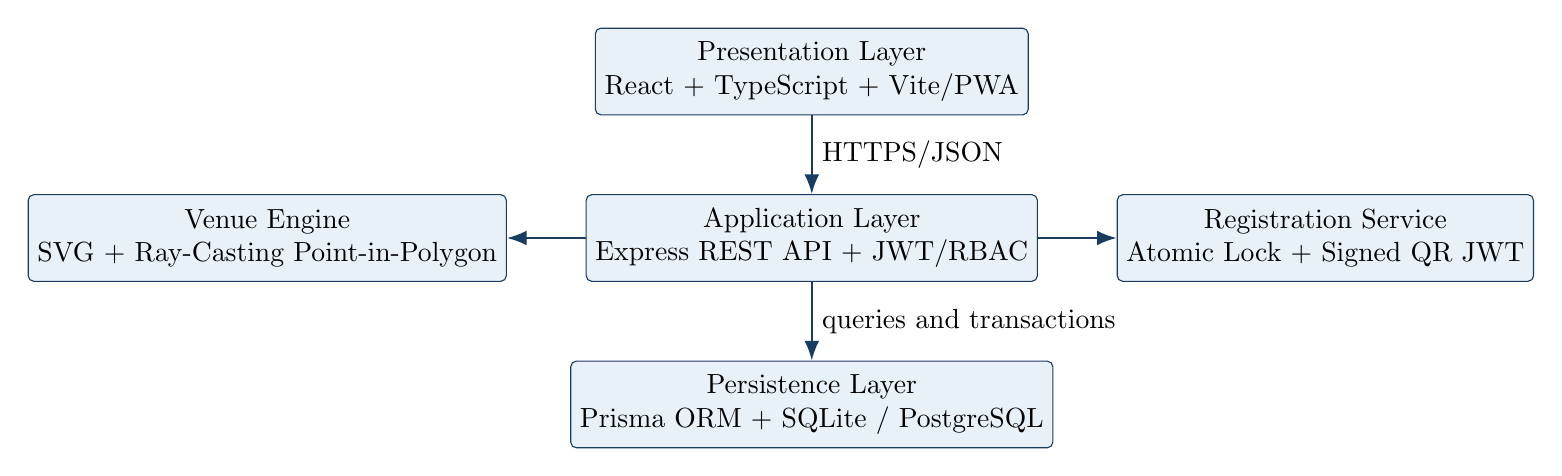
\begin{tikzpicture}[
  box/.style={draw=festblue,rounded corners=2pt,fill=lightblue,align=center,
              minimum width=4.2cm,minimum height=1.1cm},
  arrow/.style={-{Latex[length=2.5mm]},thick,draw=festblue}
]
  \node[box] (ui) {Presentation Layer\\React + TypeScript + Vite/PWA};
  \node[box,below=1.0cm of ui] (api) {Application Layer\\Express REST API + JWT/RBAC};
  \node[box,below=1.0cm of api] (db) {Persistence Layer\\Prisma ORM + SQLite / PostgreSQL};
  \node[box,left=1.0cm of api] (map) {Venue Engine\\SVG + Ray-Casting Point-in-Polygon};
  \node[box,right=1.0cm of api] (qr) {Registration Service\\Atomic Lock + Signed QR JWT};
  \draw[arrow] (ui) -- node[right]{HTTPS/JSON} (api);
  \draw[arrow] (api) -- node[right]{queries and transactions} (db);
  \draw[arrow] (api) -- (map);
  \draw[arrow] (api) -- (qr);
\end{tikzpicture}
\caption{High-level architecture of Festify}
\label{fig:architecture}
\end{figure}

\section{Actors and Major Use Cases}
The primary actors are the student, the fest administrator, and the gate volunteer or
administrator performing check-in. A student can browse events, register, view passes,
and inspect venues. An administrator can manage events and venue zones and can validate
registrations at entry. The platform itself enforces authentication, capacity, tenant
ownership, and QR-token validity.

\begin{table}[ht]
\centering
\caption{Major use cases}
\label{tab:usecases}
\begin{tabular}{p{3.1cm}p{9.5cm}}
\toprule
\textbf{Use case} & \textbf{Description}\\
\midrule
Authenticate user & Register (student self-signup) or log in, storing bcrypt hash and returning signed JWT with user role.\\
Manage events & Administrator creates, updates, and deletes event details, limits, and venue info with tenant scoping.\\
Explore venue & Student views categorized campus zones, landmarks, and performs interactive location lookups.\\
Register for event & Student submits a registration; server executes atomic transaction checking capacity and uniqueness.\\
Use QR pass & Student displays a signed pass; an authorized operator validates it at gate (preventing double check-in).\\
Manage fest tenant & Administrator writes only to the fest identified by their own account (cross-tenant calls return 403).\\
\bottomrule
\end{tabular}
\end{table}

\section{Data Model}
The database contains five central entities. A \texttt{User} stores credentials (bcrypt hash) and role. A \texttt{Fest} defines a tenant entity owned by an administrator (\texttt{ownerId}). An \texttt{Event} belongs to a Fest and administrator, storing schedule, venue, category, capacity limits, and deadlines. A \texttt{Registration} joins a student to an event and stores its signed \texttt{qrToken} and check-in status. A \texttt{VenueZone} stores a fest-owned polygon zone or point landmark.

\begin{table}[ht]
\centering
\caption{Core data entities}
\label{tab:entities}
\begin{tabular}{p{3.4cm}p{9.2cm}}
\toprule
\textbf{Entity} & \textbf{Important fields and relationships}\\
\midrule
User & id, username, password (bcrypt hash), role ('ADMIN' | 'STUDENT'); owns fests, events, and registrations.\\
Fest & id, name, startDate, endDate, branding, ownerId; parent entity for tenant events and venue zones.\\
Event & id, name, description, image, category, date, startTime, endTime, venue, maxParticipants, deadline, createdById, festId.\\
Registration & id, userId, eventId, unique qrToken, status ('REGISTERED' | 'CHECKED\_IN'), checkedInAt; unique per user-event pair.\\
VenueZone & id, name, type ('zone' | 'landmark'), category, coordinates, color, description, icon, festId; isolated per fest.\\
\bottomrule
\end{tabular}
\end{table}

\section{Technical Stack}
\begin{table}[ht]
\centering
\caption{Technical stack used in the implemented system}
\label{tab:stack}
\begin{tabular}{p{3.8cm}p{8.8cm}}
\toprule
\textbf{Technology} & \textbf{Purpose}\\
\midrule
React 18, TypeScript, Vite & Responsive student and administrator progressive web application (PWA).\\
TailwindCSS, Framer Motion & Retro-neubrutalist styling, responsive layout, and motion graphics.\\
Node.js, Express 5, tsx & REST API, middleware, and development server execution.\\
Prisma 5, SQLite & Type-safe database access and local persistence (`dev.db`).\\
JWT, bcryptjs & Signed authentication tokens and bcrypt password hashing (12 rounds).\\
SVG, Three.js, QRCode & Interactive SVG campus map, 3D pass viewer, and QR image rendering.\\
TypeScript Integration Suites & Executable automated test runners via tsx covering 49 assertions.\\
\bottomrule
\end{tabular}
\end{table}

\section{Core Registration Workflow}
The registration workflow is designed around server-side decisions rather than trusting
the client. The client requests registration for an event. The API authenticates the
student, checks the event, counts registrations, and performs the write in a serializable
Prisma transaction (`prisma.$transaction`). The unique user-event constraint (`@@unique([userId, eventId])`) prevents duplicate registrations.
On success, the API signs a JWT containing the user, event, registration, and issue-time
claims. The resulting token is rendered as a QR pass for later validation.

\begin{figure}[ht]
\centering
\begin{tikzpicture}[
  step/.style={draw=festblue,rounded corners=2pt,fill=lightblue,align=center,
               text width=3.4cm,minimum height=0.8cm},
  arrow/.style={-{Latex[length=2.3mm]},thick,draw=festblue}
]
  \node[step] (a) {Student selects event};
  \node[step,right=0.65cm of a] (b) {JWT authentication and role check};
  \node[step,right=0.65cm of b] (c) {Atomic capacity and uniqueness check};
  \node[step,below=0.75cm of c] (d) {Create registration and sign QR JWT};
  \node[step,left=0.65cm of d] (e) {Display pass in My Passes};
  \node[step,left=0.65cm of e] (f) {Authorized gate check-in};
  \draw[arrow] (a)--(b)--(c)--(d)--(e)--(f);
\end{tikzpicture}
\caption{Registration and check-in workflow}
\label{fig:registration}
\end{figure}

\section{Venue Map Workflow}
Venue data is represented in an SVG coordinate system (1000 $\times$ 700 viewBox). Polygon zones describe areas
such as stages, food courts, gates, parking, and registration points; landmarks are
represented as points. The API returns zones for a requested fest, while the locate
operation applies ray-casting point-in-polygon logic to determine the zone containing a
coordinate. Write operations require an authenticated administrator whose identifier
matches the target fest owner (`ownerId`).

\chapter{Implementation Details}
\section{Module 1: Authentication and Authorization}
The authentication module (`server/routes/auth.ts`) provides login and self-registration endpoints. New passwords are
hashed with `bcryptjs` (12 rounds) before storage. Successful authentication returns a JWT containing
user id, username, and role. The `authenticateJWT` middleware rejects missing or
invalid tokens, while `requireAdmin` protects administrator-only operations.
Self-service registration (`POST /api/auth/register`) enables student signups while explicitly blocking `ADMIN` role self-creation with HTTP 403; administrator accounts are provisioned through controlled seed or administrative flows. Canonical token storage on the frontend is unified on `festify_token` and `festify_role`.

\section{Module 2: Event Management}
Administrators can create, read, update, and delete events (`server/routes/events.ts`). Event records include the
name, description, category, date, start and end time, venue, maximum participants,
registration deadline, rules, prizes, contact info, and status.
Cross-tenant event mutation protection ensures that an administrator attempting to update (`PUT`) or delete (`DELETE`) an event owned by another admin receives an explicit `403 Forbidden` response. Public event listings return dynamic `remainingSeats` and `registeredCount` calculations.

\section{Module 3: Interactive Venue Map}
The venue module (`server/routes/venue.ts`) exposes tenant-scoped zone retrieval and protected zone creation.
The frontend (`src/components/VenueMap.tsx`) renders the campus plan as an interactive SVG with category filters,
pan-and-zoom controls, and selected-zone inspection. The backend point-in-polygon algorithm implements ray-casting ray intersections over polygon vertices to determine hit/miss location results deterministically.

\section{Module 4: Registration and QR Passes}
Registration is implemented as a protected API operation (`server/routes/registrations.ts` and `events.ts`). It rejects unauthenticated
requests, duplicate user-event pairs, and requests that exceed the configured event
capacity. The database transaction is serializable so two simultaneous requests for the
last available seat cannot both succeed. The QR token is signed with the server secret,
and check-in (`POST /api/registrations/:registrationId/checkin`) verifies the token signature before setting status to `CHECKED_IN` and recording `checkedInAt`. Re-check-in attempts return HTTP 400.

\section{Module 5: Frontend Experience}
The frontend contains landing, authentication modal, student, and administrator views. The
student view supports event discovery, event details, venue exploration, registration,
pass display, and interactive 3D pass inspection. The administrator dashboard supports event administration, venue zone creation, and gate check-in scanning simulation. The application includes PWA
manifest and caching support, responsive layouts, and unified localStorage key management.

\section{Security and Tenant Isolation}
Tenant isolation is enforced at the route boundary. An administrator's user identifier
acts as the fest owner identifier for venue and event operations. Before an admin writes
to a target fest or event, the API compares the authenticated identity with the target owner.
The venue and events integration suites verify that data created for one fest is not returned for
another fest and that cross-tenant writes receive HTTP 403. Authentication tests verify missing-token, invalid-token, role, password, and self-signup restrictions across 30 dedicated assertions.

\chapter{Results and Evaluation}
\section{Testing Methodology}
Testing focused on automated integration test suites executed directly against the API layer and database:
\begin{itemize}
  \item \textbf{Authentication integration suite (\texttt{server/auth.test.ts}):} 30 assertion checks covering student signup (201), token verification, bcrypt hash storage, password verification, duplicate username rejection (409), admin self-signup block (403), short password rejection (400), valid/invalid login, seeded user login, `authenticateJWT` pass/fail, and `requireAdmin` RBAC enforcement.
  \item \textbf{Event security suite (\texttt{server/events.test.ts}):} 5 assertion checks covering event creation, authorized update, cross-tenant update rejection (403), cross-tenant deletion rejection (403), and authorized deletion.
  \item \textbf{Venue integration suite (\texttt{server/venue.test.ts}):} 7 assertion checks covering tenant-scoped zone reads/writes, cross-tenant write rejection (403), ray-casting polygon point-in-polygon hit/miss logic, and unauthenticated rejection (401).
  \item \textbf{Registration concurrency suite (\texttt{server/registration.test.ts}):} 7 assertion checks covering event capacity limits, simultaneous last-seat concurrent requests (1 pass 201, 1 fail 400), signed QR token generation, token payload verification, duplicate registration prevention, gate check-in status update, and double check-in rejection.
\end{itemize}

\section{Performance and Functional Metrics}
The executable test suites yielded 100\% pass rates across all 49 documented assertion checks.

\begin{table}[ht]
\centering
\caption{Implemented system integration test results}
\label{tab:results}
\begin{tabular}{p{5.1cm}p{2.4cm}p{4.9cm}}
\toprule
\textbf{Area} & \textbf{Result} & \textbf{Verified behavior}\\
\midrule
Authentication suite & 30 checks passed & Signup, login, bcrypt hashing, JWT, invalid access, and RBAC.\\
Event security suite & 5 checks passed & Event lifecycle and cross-tenant mutation write isolation (403).\\
Venue integration suite & 7 checks passed & Tenant isolation, ray-casting polygon locate, 401 rejection.\\
Registration concurrency suite & 7 checks passed & Capacity lock, QR claims, duplicates, check-in, re-check-in.\\
Total assertion checks & 49 checks passed & Core backend security, concurrency, and workflow behavior.\\
\bottomrule
\end{tabular}
\end{table}

\section{Analysis}
The implemented system meets the principal functional objectives for a production-ready prototype. The authentication suite demonstrates that passwords are stored as bcrypt hashes and that roles are strictly enforced. The venue and event security suites prove that an administrator cannot update or delete resources belonging to another fest tenant. The registration suite demonstrates concurrent safety: when two simultaneous requests arrive for the final available seat, exactly one request succeeds (201) while the other receives an event-full response (400).

The results also delineate the current deployment boundary. The prototype operates locally on SQLite for zero-dependency execution, with a structured PostgreSQL/PostGIS raw migration script provided in `prisma/migrations/20260917000000_postgis_fest_migration/` for production scale-out.

\chapter{Conclusion}
\section{Summary of Work}
Festify was developed as a reusable multi-tenant college fest management platform. The project combines a responsive React PWA with a protected Express REST API and Prisma-backed persistence. The implemented system supports user accounts, role-based access control, fest tenants, events, tenant-owned venue zones, capacity-locked registration, signed QR passes, and gate check-in validation.

\section{Key Findings}
\begin{enumerate}
  \item Server-side capacity locks inside serializable database transactions (`prisma.$transaction`) are essential to prevent race-condition overbooking under concurrent student requests.
  \item Multi-tenant isolation must be enforced and tested at the API boundary; cross-tenant write operations return explicit HTTP 403 Forbidden responses.
  \item Cryptographically signed JWT QR tokens allow fast gate verification, while server-side check-in endpoints prevent pass reuse.
  \item A multi-tenant model allows multiple college fests to be hosted without modifying frontend code or rebuilding backend schemas.
\end{enumerate}

\section{Future Work and Recommendations}
The following extensions are recommended:
\begin{enumerate}
  \item Execute the included PostGIS migration (`prisma/migrations/20260917000000_postgis_fest_migration/migration.sql`) to move from SQLite to PostgreSQL for production spatial indexing.
  \item Connect the frontend check-in view to native HTML5 WebRTC camera APIs for live mobile QR barcode scanning.
  \item Activate the Socket.IO real-time event broadcasting and Redis crowd telemetry seams established in `AdminDashboardView.tsx`.
  \item Introduce refresh-token rotation, secrets management, and automated production CI/CD pipelines.
\end{enumerate}

\section{Final Remarks}
Festify demonstrates how college fest coordination can be modernized through robust data modeling, explicit authorization boundaries, transactional workflows, and comprehensive automated test suites. The system provides a solid foundation for multi-tenant college event management.

\begin{thebibliography}{9}
\bibitem{react} Meta Open Source, ``React Documentation,'' 2026.
\bibitem{express} Express.js, ``Express - Node.js Web Application Framework,'' 2026.
\bibitem{prisma} Prisma, ``Prisma ORM Documentation,'' 2026.
\bibitem{jwt} M. Jones, J. Bradley, and N. Sakimura, ``JSON Web Token (JWT),'' RFC 7519, 2015.
\bibitem{owasp} OWASP Foundation, ``OWASP Application Security Verification Standard,'' 2025.
\bibitem{projectstatus} Festify Team, ``Festify Project Status and Technical Documentation,'' project repository, 2026.
\end{thebibliography}

\end{document}
